%%%%%%%%%%%%%%%%%%%%%%%%%%%%%%%%%%%%%%%%%%
	\begin{frame}[plain]
	 	\frametitle{LSI: A quick example}
\begin{equation}
 U =
\begin{pmatrix}
 -0.45 & -0.30 & 0.57 & 0.58 & 0.25 \\
 -0.13 & -0.33 & -0.59 & 0 & 0.73 \\
 -0.48 & -0.51 & -0.37 & 0 & -0.61 \\
 -0.70 & 0.35 & 0.15 & -0.58 & 0.16\\
 -0.26 & 0.65 & -0.41 & 0.58 & -0.09 \end{pmatrix}
\end{equation}
\begin{equation}
 \Sigma =
\begin{pmatrix}
 2.16 & 0 & 0 & 0 & 0\\
 0 & 1.59 & 0 & 0 & 0\\
 0 & 0 & 1.28 & 0 & 0\\
 0 & 0 & 0 & 1.00 & 0\\
 0 & 0 & 0 & 0 & 0.39 \end{pmatrix}
\end{equation}
\begin{equation}
  V^{T} = 
\begin{pmatrix}
 -0.75 & -0.28 & -0.20 & -0.45 & -0.33 & -0.12\\
 -0.29 & -0.53 & -0.19 &  0.63 &  0.22 &  0.41\\
  0.28 & -0.75 &  0.45 & -0.20 &  0.12 & -0.33\\
  0    &  0    &  0.58 &  0    & -0.58 &  0.58\\
 -0.53 &  0.29 &  0.63 &  0.19 &  0.41 & -0.22 \end{pmatrix}
\end{equation}
	\end{frame}
%%%%%%%%%%%%%%%%%%%%%%%%%%%%%%%%%%%%%%%%%%
\begin{frame}[plain]
\frametitle{LSI: A quick example}
\begin{equation}
 \Sigma_{2} =
\begin{pmatrix}
 2.16 & 0.00 \\
 0.00 & 1.59 \end{pmatrix}
\end{equation}
\\
\begin{equation}
A_{2} = \begin{pmatrix}
    1.0199 &   0.0060 &   1.0112 &   0.0095 &   0.0069 &  -0.0047 \\
    0.0004 &   1.0057 &  -0.0046 &   0.0009 &   0.0033 &   0.0052 \\
    1.0062 &   1.0063 &  -0.0016 &   0.0052 &   0.0094 &   0.0006 \\
    0.9933 &   0.0025 &  -0.0140 &   1.0045 &   1.0064 &  -0.0039 \\
   -0.0069 &  -0.0071 &  -0.0059 &   1.0021 &  -0.0011 &   1.0084 \end{pmatrix}
\end{equation}
\\
\begin{equation}
\|A - A_{k}\|_{2} = 1.28
\end{equation}
\\
\begin{equation}
\Sigma_{2} V_{2}^{T} = \begin{pmatrix}
 -1.62 & -0.60 & -0.44 & -0.97 & -0.70 & -0.26\\
 -0.46 & -0.84 & -0.30 &  1.00 &  0.35 &  0.65 \end{pmatrix} 
\end{equation}
\end{frame}
%%%%%%%%%%%%%%%%%%%%%%%%%%%%%%%%%%%%%%%%%%
\begin{frame}[plain]
\frametitle{LSI: A quick example}
\begin{equation}
q = \begin{pmatrix}0\\1\\0\\0\\0\end{pmatrix}
\end{equation}\
\\
\begin{equation}
q_{k} = \begin{pmatrix}-0.06\\-0.21\end{pmatrix}
\end{equation}
\end{frame}
%%%%%%%%%%%%%%%%%%%%%%%%%%%%%%%%%%%%%%%%%%
\begin{frame}[plain]
\frametitle{LSI: A quick example}
\begin{center}
  \begin{figure}[H]
    \centering
    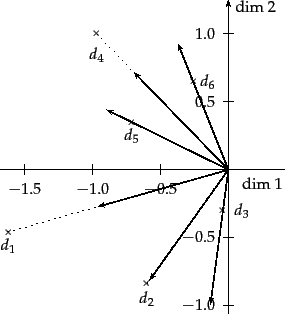
\includegraphics[width=5cm]{space.png}
    \label{fig:spaces}
  \end{figure}
\end{center}
\end{frame}

